%%
%% neuralfields.tex
%% 
%% Made by jjfigueredou
%% Login   <jjfigueredou@fctp-jjfu>
%% 
%% Started on  Sun Oct  5 12:26:22 2008 jjfigueredou
%% Last update Sun Oct  5 12:26:22 2008 jjfigueredou
%%
\documentclass[conference]{IEEEtran}
%\documentclass[preprint]{sigplanconf}
\usepackage{stmaryrd}
\usepackage{amsfonts}

\usepackage[latin1]{inputenc}
\usepackage[numbers]{natbib}
\usepackage[english]{babel}
\usepackage{graphicx}
\usepackage{algorithm}
\usepackage{algorithmic}
\usepackage{amsmath}

\hyphenation{op-tical net-works semi-conduc-tor IEEEtran}

\IEEEoverridecommandlockouts    % to create the author's affliation portion
                % using \thanks

\textwidth 178mm    % <------ These are the adjustments we made 10/18/2005
\textheight 239mm   % You may or may not need to adjust these numbes again
\oddsidemargin -7mm
\evensidemargin -7mm
\topmargin -6mm
\columnsep 5mm


\begin{document}

\title{\ \\ \LARGE\bf Applying Neural Fields to the Stability Problem
  of an Inverted Pendulum as a Simple Biped Walking Model \thanks{Juan
    Figueredo and Jonatan G�mez are with the Department of Systems and
    Industrial Engineering, National University of Colombia, Bogot�,
    Colombia (email: \{jjfigueredou,jgomezpe\}@unal.edu.co).}}

\author{Juan Figueredo and Jonatan G�mez}

\maketitle

\begin{abstract}
  This paper proposes a control architecture based on neural fields
  for a relatively complex and unstable dynamical system. The neural
  field model is capable of addressing goal-based planning problems
  and has properties, like embedding in an Euclidean space and linear
  stability, that potentially make it well-fitted for dynamic control
  tasks. The neural field control architecture is tested with the
  inverted pendulum problem. The cart-and-pole inverted pendulum is
  used as a simple biped walking model, where the cart models the
  center of pressure and the pole models the center of mass. The
  parameterized (i.e. non-evolved) neural field control architecture
  is compared against an evolved recurrent neural field controller
  applied to the same control task. The non-evolved neural field
  controller performs, in the simulation, better than the evolved
  recurrent neural network controller. Furthermore, the neural field
  has a spatial representation which allows an easy visualization of
  its field potentials.
\end{abstract}

\section{Introduction}
%% Intro outline
% 1. What is artificial life 2. What is the artificial life approach
% to evolutionary robotics 3. What has been done in biped robotics
% (detail static and dynamic control) 4. Why goal-oriented control is
% lacking but desirable 5. Why neural fields for goal-oriented control
% and (the little) previous work 6. Why biped walking as
% inverted-pendulum and previous work. Brief comparison with
% reference-tracking control.  7. Previous work on inverted pendulum
% control with computational intelligence methods emphasizing RNNs
% 8. Outline of contents
%%

Artificial life aims to devise and study those emergent phenomena that
give complex attributes to the living beings, like self-organization,
cooperation, self-reproduction and adaptation, among others
\cite{Bedau92Philosophical}. It focuses on the generation of behavior
from a biological, bottom-up perspective that relies on evolution,
development and learning \cite{Dyer94Toward}.

Following a pure artificial life approach to evolutionary robotics
\cite{Nolfi04Evolutionary}, it is expected that complex behaviors of
simulated agents emerge by local interactions of elements. These
interactions form a complex dynamical system which is the generator of
behavior and is capable of some form of adaptation or
evolution. Examples of such dynamical systems are recurrent neural
networks \cite{Huelse04Structure} and feed-forward neural networks
\cite{Stanley02Evolving}.

One of the tasks in evolutionary robotics is the emergence of motion
control and planning capabilities of biped walking agents.

In biped robotics, the methods based on computational intelligence for
planning and control have shown to be able to achieve static stability
\cite{Kun97Adaptive} (stability omitting accelerations), dynamical
stability \cite{Nakanishi2004b,Komatsu05Dynamic} (stability taking
into consideration accelerations), achieve simple control structures
\cite{Huelse04Structure}, and tolerate perturbations
\cite{Juang02Intelligent}. Nonetheless, in order to obtain emergent
complex behaviors, it is needed an architecture capable of following
simple behavioral goals, and composing them into complex
behaviors. This approach differs from the normal reference-tracking
control, where the goal is to follow a reference signal or, similarly,
to minimize an error signal \cite{Chen93Analog}.

The cart-and-pole inverted pendulum model, and some extensions of it,
has been used previously to give insight on walking patterns without
all the complexities of handling several joints
\cite{Kajita91Study,Kajita92Dynamic,Sugihara03Contact}. In this
approach, the cart base models the center of pressure (CoP), the pole
mass models the center of mass (CoM), and the link joining both models
a conceptual line between the CoM and the CoP.

The control architecture applied in this paper to the biped walking
problem follows the method of planning and control by means of neural
fields \cite{Bergener99Complex}. The neural field model, as noted in
the article by Bergener et al., has the potential to address
goal-based planning problems, so we are here interested on its
capability to solve dynamic control problems, and specifically, on its
capability to address control tasks on unstable systems. The
parameterized (i.e. non-evolved) neural field control architecture is
compared against an evolved recurrent neural field controller applied
to the same cart-and-pole control task

This is a first attempt (to the authors' knowledge) to evaluate neural
fields for solving a control problem for an unstable plant, and
specifically for solving the inverted pendulum control
problem. However, there is a wide range of methods that have been
applied to the inverted pendulum problem both based on computational
intelligence (e.g. \cite{Anderson89Learning, Bardossy95Fuzzy,
  Moriarty96Efficient, Zhang02recurrent}) and based on control theory
techniques (e.g. \cite{Kajiwara99LPV, Huang00Control,
  Chang02self-tuning}).

This paper is divided in seven sections. In section II, some
preliminaries on computational intelligence are presented, mainly in
the area of neural fields and recurrent neural networks, which is the
main focus of the article, and in the area of evolutionary
computation. In section III, the control problem is detailed. In
section IV, the neural field control architecture is presented and a
strategy for its parameterization by evolution is mentioned. In
section V, the recurrent neural network controller and its evolution
is shown. In section VI, the experimental process and results are
presented and discussed. Finally, in section VII, some conclusions and
future work are presented.


\section{Preliminaries on Computational Intelligence}
\subsection*{Recurrent Neural Networks}
Artificial neural networks are a connectionist computing scheme
inspired by brain neural layout at cellular level. It is based on
simple computing structures, neurons, which have several inputs and a
single output. Many different topologies have been proposed. Here,
special attention is paid to recurrent neural networks and neural
fields.

We used the recurrent neural networks model, as it is presented in
\cite{Haykin98Neural}, that can by described in equation \ref{eq:rnn}.

\begin{equation}
  \label{eq:rnn}
  \begin{split}
    x_{r}(n+1)&=\Psi (W_ax_{r}(n)+W_bu_{r}(n)) \\
    y_{r}(n)&=Cx_{r}(n)
  \end{split}
\end{equation}

Here, $x_{r}$ is the $1 \times q$ system state vector at $n$, $\Psi$
is a diagonal function with domain and co-domain $R^q$ corresponding
to activation function, $u_{r}$ is the $1 \times m$ input vector at
$n$, the $q \times q$ matrix $W_a$ represents the connection weights
between neurons, and the $q \times (m+1)$ matrix represents the
connection weights between input nodes and neurons, including a bias
term. Also, $y_{r}$ is the neural output vector of the neural net, and
$C$ is a $p \times q$ matrix of linear combination from the neurons to
the outputs.

Recurrent neural networks present a dynamic behavior because of its
memory, that is, each state depends of the previous state in such a
way that a difference equation arises. There is not a notion of
neighborhood in this model. The interaction between neurons and inputs
is given by matrices of weights and there is no need to embed the
neurons in a metric space.

\subsection*{Neural Fields}
Neural fields, on the other hand, arise as a tissue level model of
neural populations in brain. They have been proposed by Wilson and
Cowan \cite{Wilson72Excitatory} and detailed by Amari
\cite{Amari77Dynamics} in the particular case of lateral
inhibition. In this model, a neural population is considered a
continuum in which dynamical evolution is driven by mean activation
potentials. The field potential is evaluated in each place and
affected by the neighborhood of that place, according to a so-called
mexican hat function (as noted by Coombes \cite{Coombes05Waves} better
called wizard hat function), in which close neighbors act as exciters
and distant ones act as inhibitors. The elements on the field are
embedded into a metric space, usually a one-dimensional or
two-dimensional Euclidean space. The mathematical formulation for the
one-dimensional case is described in equation \ref{eq:neuralfield}:

\begin{equation}
  \label{eq:neuralfield}
  \frac{1}{\alpha}
  \dot{u}(x)=-u(x)-h+s(x)+\int_{-\infty}^{\infty}{w(x,x')\sigma(u(x'))dx'}
\end{equation}
Where $\alpha$ is a temporal constant of synaptic decay rate, $u(x)$
is the average membrane potential of the neurons located at position
$\psi$ at time $t$ (where $\psi$ is supposed to be 1-dimensional and
the time is omitted for readability). The average intensity of
connection from neurons at $\psi$ to neurons at $x'$ is modeled with
$w(x,x')$, which is a kernel (not necessarily positive definite) over
the space where the field is embedded. The function $f(\cdot)$ is the
saturating output, which is monotonically nondecreasing. The deviation
of the average stimulation potential at place $\psi$ at time $t$ is
represented by $s(x)$, and $h=\bar{s}-r$ is the sum of the average
stimulation potential and the resting potential.

Recurrent neural networks and neural fields have some important
differences. In recurrent neural networks the relation among the
neurons is arbitrary and discrete. On the other hand, in neural fields
the relation among the (infinite) elements is continuous and is meant
to be related to the neighborhood of each element. While a discrete
variation of the neural field model (which is needed for simulation)
makes the difference related to continuity less substantial, the
connection scheme in the neural field is still more restrictive than
in the recurrent neural network. Nevertheless, this additional
restriction allows an easier visualization of neural fields by
plotting the field potentials over the Euclidean space. Besides, in
the neural field model equation, the first right hand element assures
and stable homogeneous behavior in the simplified linearized form.

\subsection*{Evolutionary algorithms}
Evolutionary algorithms are a set of population-based heuristic search
and optimization techniques \cite{Fogel99Evolutionary}. They maintain
a population, and apply a set of operators or transformations over its
members. Those operators are typically inspired on biological
evolution and usually include selection, reproduction and mutation,
among others. Such operators are dependent of the evaluation of a
performance function called fitness function. Generally, fitness
function evaluation may include, from a simple numerical evaluation,
to a complex simulation, in order to get the performance criterion
which its optimization is pursued.

The pseudo-code of a general evolutionary algorithm is as follows:

\algsetup{indent=2em}
\begin{algorithm}[h!]
  \caption{$Evolutionary Algorithm$}\label{alg:factorial}
  \begin{algorithmic}[1]
    \STATE $P \leftarrow$ Generate initial population of size $N$
    \STATE Evaluate fitness for each individual in $P$ \REPEAT \STATE
    $P' \leftarrow$ Apply operators to $P$ \STATE Evaluate fitness for
    each individual in $P'$ \STATE $P \leftarrow$ Select $N$
    individuals in $P'$ according to a selection scheme
    \UNTIL{Termination condition is met}
  \end{algorithmic}
\end{algorithm}

The most predominant form of an evolutionary algorithm is embodied by
genetic algorithms \cite{Holland92Adaptation,
  Goldberg89Genetic}. Their most frequent genotypical representation
is a bit sequence, although other representations can be used. Usually
genetic algorithms are implemented with a generational replacement of
population, but in some situations it is useful to conserve a small
set of the better individuals across generations in a steady-state
replacement.

\section{The Stability Problem Model}
\label{sec:model}

The model used consists of an approach to biped walking based on a
inverted pendulum (cart-and-pole) system in which the pendulum
equilibrium is looked for. Nonetheless, supposing that the pendulum
mass represents the body center of mass, it is proposed that is
reasonable to expect a system with its sole function being to
stabilize the body \cite{Huang00Control,Anderson89Learning}. For
example, if we where to devise a navigation system, it could have as
purpose to carefully perturb the first controller, in such a way that
the stabilizing controller moves the cart to the desired position.

\subsection*{Dynamic Model}
The dynamic model used, in mathematical terms, is expressed in the
equations \ref{eq:nf-simp} and \ref{eq:nf-simp2}:

\begin{align}
  \label{eq:nf-simp}
  \ddot{x}&=\frac{F+ml\dot{\theta}^2\sin\theta-mg\cos\theta\sin\theta}{M+m\sin^2\theta}\\
  \label{eq:nf-simp2}
  \ddot{\theta}&=\frac{(M+m)g\sin\theta-F\cos\theta-ml\dot{\theta}^2\sin\theta\cos\theta}{l(M+m\sin^2\theta)}+\frac{\tau}{ml^2}-\frac{\dot{\theta}}{2}
\end{align}
Where $x$ here is the linear position, $\theta$ is the angular
position, $M$ is the pendulum mass (located at the outer side), $m$ is
the cart mass, $l$ is the pendulum length and $g$ is the gravity
acceleration. It is included in the model a viscous friction for the
rotation.


This model consists of four state variables and a high non-linearity
as it departs from equilibrium points. It is worth noting that the
wanted equilibrium point is in fact unstable.


\section{Neural Fields for Control and Planning}

\subsection*{Properties}
\label{sec:properties}
For the purpose of control and planning we need some particular
requirements on the neural fields. The first one is to have a
preprocessing over the input obtained from the sensors, so that there
is a closed loop where the representation of inputs has an appropriate
form. This mechanism alone (a particular form for the inputs) has
shown to be enough for the robot ARNOLD to navigate in the plane with
obstacles \cite{Bergener99Complex}.

A second requirement is to be able to modify the connection kernel so
that it can be suitable to solving complex control problems. While in
this paper it is not applied a process of adaptation or evolution to
the neural field, the adaptation capability is essential viewed from
the perspective of artificial life. In order to achieve that, we will
consider that the connection kernel $w(y)$ is a symmetric function
(i.e. $w(y)=w(-y)$). Notice that it is also a 2-power Lebesgue
integrable function so it belongs to $L^2$. It can be shown that a sum
of an arbitrary number of kernel functions will also be a kernel
function. In this way, we have a inner-product defined by the Lebesgue
measure, described in equation \ref{eq:eq-l2}:

\begin{equation}
  \label{eq:eq-l2}
  \langle f,g \rangle_{L^2} = \int_{R}{f\cdot g d\mu}
\end{equation}

The defined space, with its measure, conforms a Hilbert space, and
therefore is complete and metrizable. It also gives a notion of sum,
and scalar product, as shown in equations \ref{eq:eq-leb-opers}:
\begin{align}
  \label{eq:eq-leb-opers}
  (f+g)(x)=&f(x)+g(x) \\
  (\lambda f)(x)=&\lambda f(x)
\end{align}
Those properties define and space with its operators which can be used
to apply an evolutionary algorithm, or another adaptation technique,
by varying the kernel function of the neural field. Nonetheless, it
should be noted that, in this paper, the kernel parameterization is
directly made, and therefore it is not performed by an adaptation or
evolution technique

In this sense, the parameters for a two layer architecture (i.e. with
input and processing fields) are the connection kernels between the
input field and the processing field, and the recurrent connections of
the processing field with itself.

If the connection kernels are considered isotropic and homogeneous
along each field, each connection kernel can be represented as an
array of $N$ values from $w(0)$ to $w(p)$ with homogeneous spacing,
using its symmetry. This way, for an equal boundary radius for all the
kernels, and a 3-layered architecture, there are $3N$ real values in
the parameter set. As can be seen, the number of parameters does not
have a direct relation with the simulation size of the neural fields
(the number of discrete points used), in contradistinction with
recurrent neural networks, where the number of parameters depends on
the number $n$ of neurons with a polynomial order $O(n^2)$.

A third requirement is the suitability to simulation of the neural
field. This is not an inherent restriction for it to be physically (or
biologically) plausible, but to be implementable on a computer. We
will take a discrete form of the equation \ref{eq:nf-simp}, described
in equation \ref{eq:nf-disc}:


\begin{equation}
  \label{eq:nf-disc}
  \tau \dot{u}_i=-u_i+\sum_{x_j \in B_p(x_i)} {w\left(x_i,x_j\right)
    f\left( u_j \right)}+S(x_i,t)
\end{equation}

Here we denote $u_i=u(x_i,t)$. We replace the integral for a sum over
the point included inside a finite neighborhood (ball) around $x_i$
with radius $p$. Time is considered continuous, and the computation of
the dynamical system behavior is evaluated with a fourth-order
Runge-Kutta method. It should be noted that the previous equation can
be applied to the $n$-dimensional case without any modification.

\subsection*{Control Architecture} 
The proposed control architecture based on the neural fields has three
basic elements.

The sensor reads the states from the plant and also their derivatives
(computed from the dynamical equation of the plant). In particular,
the sensor used for the neural field controller is rather simple,
taking the values of the angular-related states (i.e. angular position
and angular velocity) as feedback.

The input layer consists of a simple neural field without natural
dynamics and produces a spatial codification of the sensed values. For
the problem at hand, we use a finite one-dimensional neural field,
where a sensed input with value zero maps to the center point of the
field, and other values are correspondingly coded in other (positive
or negative) positions. Angular position values are coded as local
potentials with value $u(x)=1$ and angular velocities as local
potentials with value $u(x)=k_\omega$, where $0 \le k_\omega < 1$. It
is worth noting that the sum between input states is performed
directly by the neural field dynamics.

The processing layer is a more typical neural field which has inner
dynamics given by the equation \ref{eq:nf-disc}. Each position of the
processing field takes as input, both the field potentials of the
processing field, and the field potentials of the input
field. Therefore, besides its natural dynamics, the processing layer
receives the inputs from the input field filtered by the kernel
operator. The kernel operator used here is a Wizard Hat Function with
the expression shown in equation \ref{eq:wizard-hat}:

\begin{equation}
  \label{eq:wizard-hat}
  w(x_i,x_j)=ke^{-(x_i-x_j)^2/\delta^2}-H_0
\end{equation}

The additional term on the eq. \ref{eq:nf-disc} $S(x_i,t)$ is used
only as the uniform and static resting potential, that is
$S(x_i,t)=-r_p$.  The firing rate function $f(u_i)$ is simulated as a
simple Heaviside function.

The output is processed taking the position with highest activation on
the processing filtered by another wizard-hat function, and decoding
it to a value.

Figure \ref{fig:nf-control} shows the input and output layers (in the
2-dimensional case for generality) and the participation on the
potential of a single element in the processing (or main) layer from
the elements in the same layer and in the input layer.


\begin{figure}[t]
  \centering
  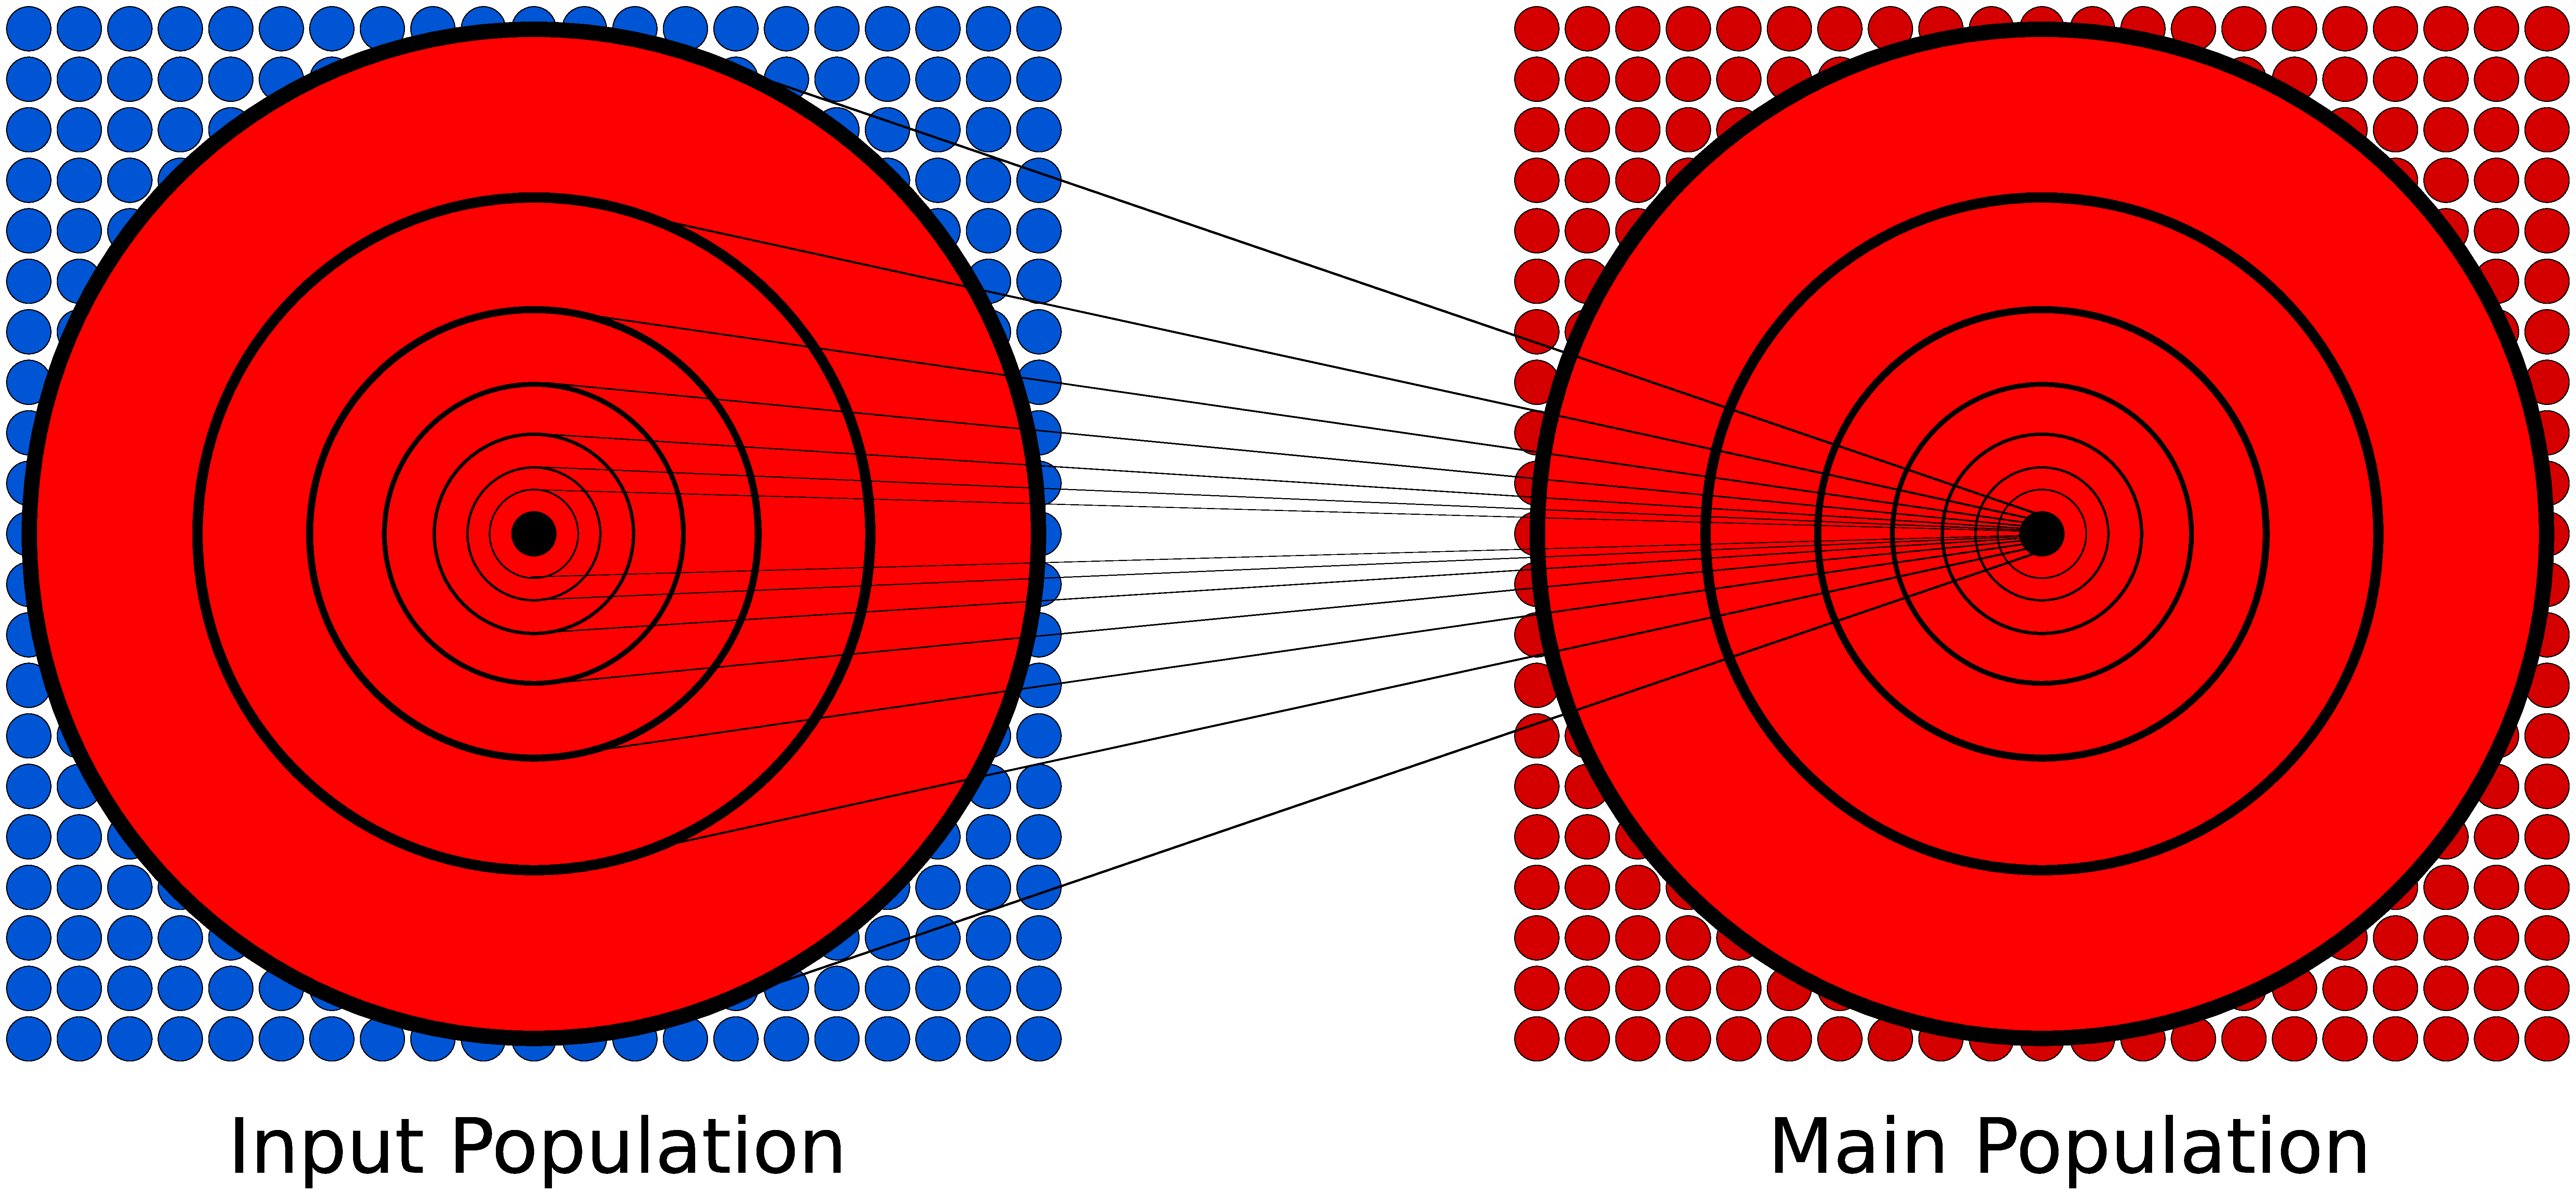
\includegraphics[width=7cm]{fieldsGaussians.eps}
  \caption{Neural fields for stability control (feedback with the
    plant not shown). \label{fig:nf-control}}
\end{figure}

\section{The RNN Controller Architecture}
\label{sec:rnncontroller}
% \subsection*{RNN Controller Architecture for Comparison}
The proposed architecture for the recurrent neural network controller
has two expert recurrent networks, whose interaction will achieve
positioning and equilibrium as well.

It is applied a preprocessing stage for the input neurons, so the
actual values are not used and instead the inputs are mapped to 3
fuzzy sets. In this way, the stability controller only has 3 inputs,
while the positioning controller has 6, corresponding to the same 3
inputs previously described and another 3 due to the fuzzy mapping of
the error signal. All neurons are interconnected and the first one of
them is selected as output without loss of generality. The neural
network topology for the first controller (stability) is shown in the
figure \ref{fig:rnn-arch}.

\begin{figure}[t]
  \centering
  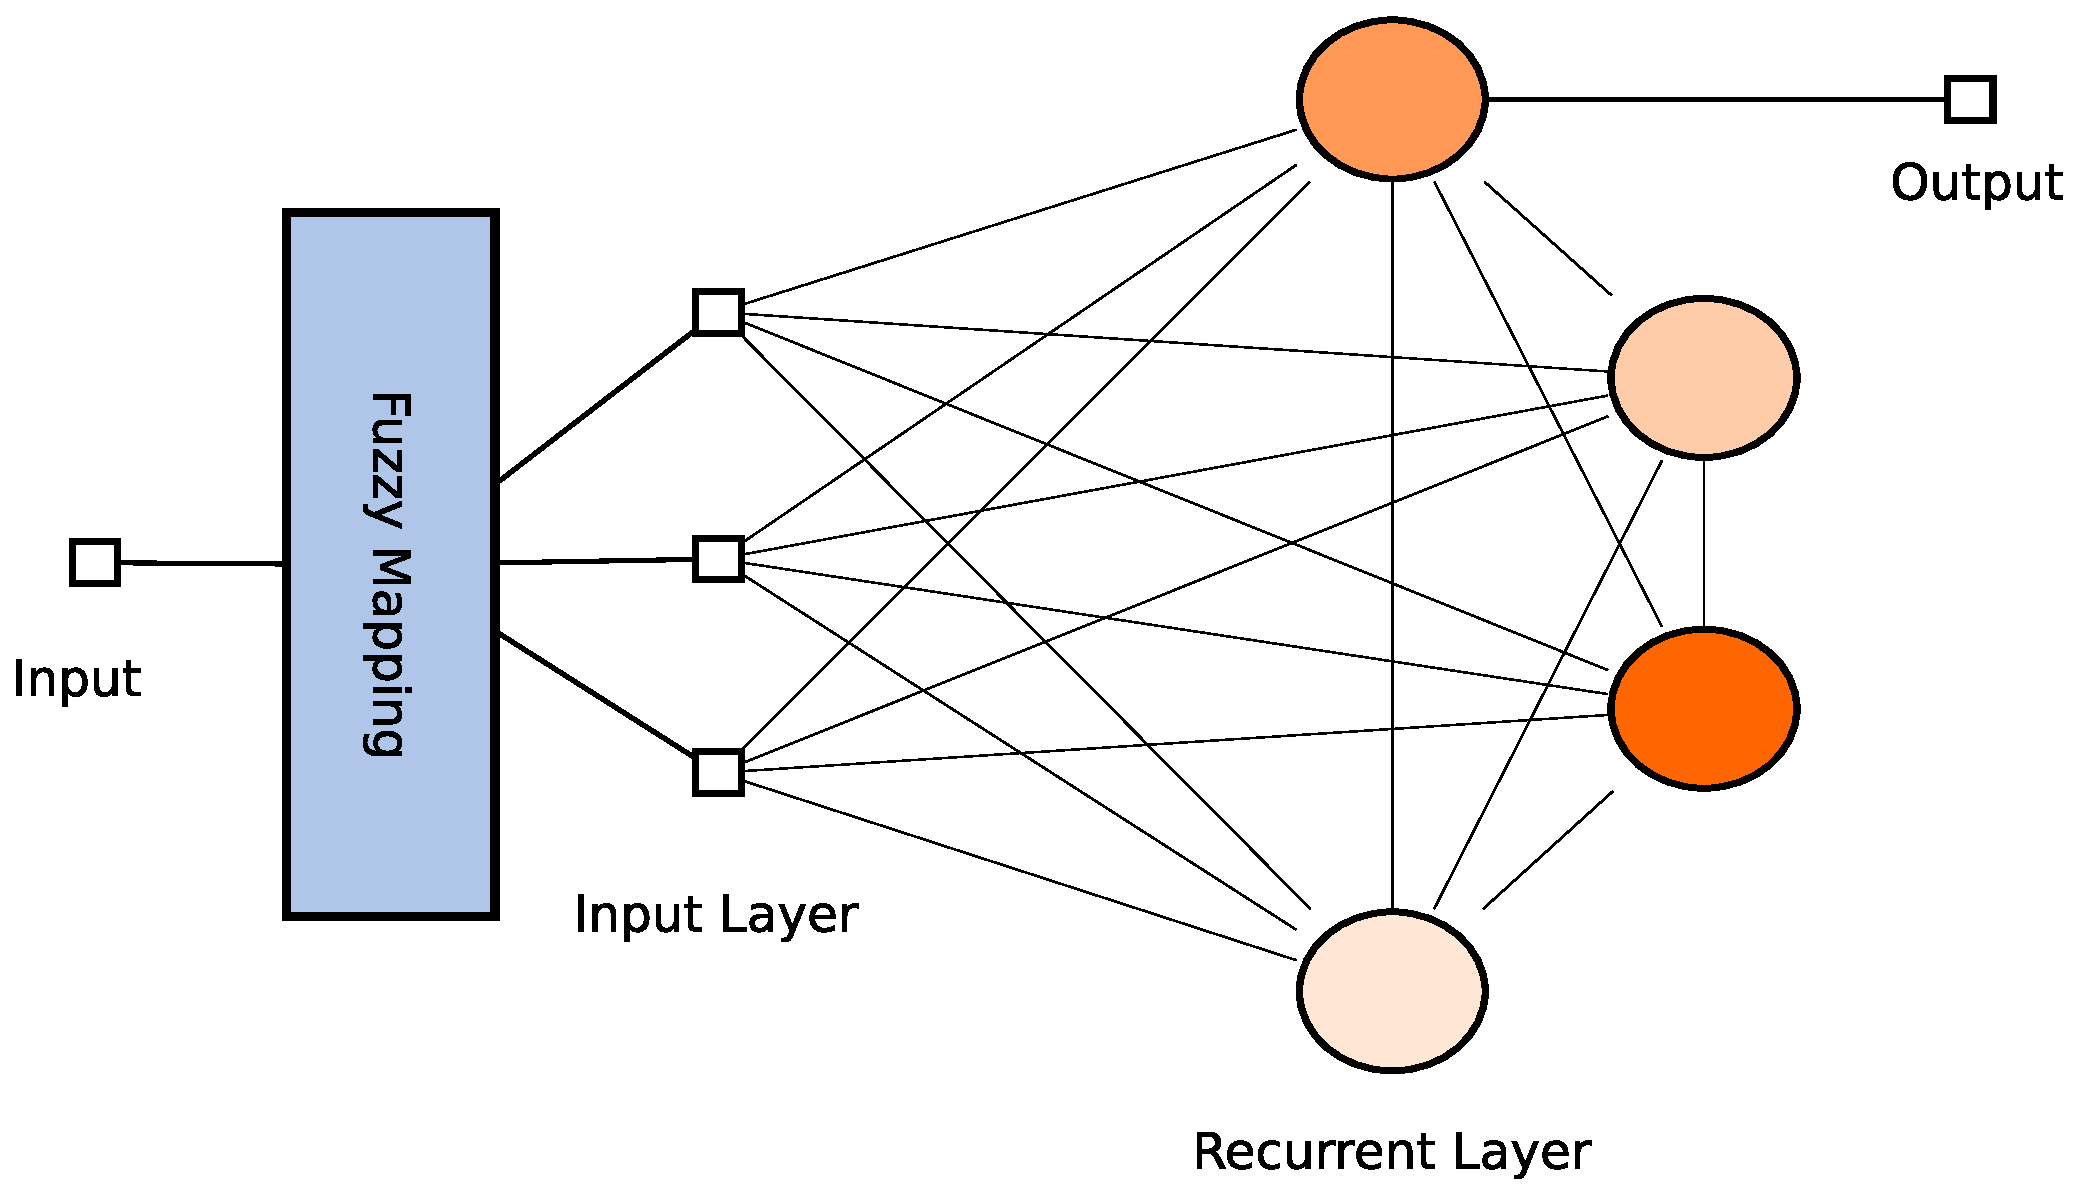
\includegraphics[width=7cm]{rnn.eps}
  \caption{Neural net for stability control including fuzzy
    mapping \label{fig:rnn-arch}}
\end{figure}

\subsection*{Evolutionary Algorithm Structure for the RNN Controller}
It is expected, based on the approach of artificial life to
evolutionary robotics \cite{Nolfi04Evolutionary}, that the sequential
and cooperative evolution of elements with biological similarity leads
to an specialization in the process of stabilization and positioning
(despite the antagonistic individual goals of each controller because
of the interest of the positioning controller to maximize also the
global performance).

As said, the two steps are executed sequentially, taking the best
individual of the first step to collaborate with the individual
evolved in the second step.

Aiming to obtain a fixed length representation and limit the problem
dimensionality, a totally connected model of order $Q$ is used. Any
network with an order equal or lesser than $Q$, and with total or
partial connections, can be represented by the proposed model by the
addition of activating/deactivating elements for neurons and
connections. Therefore, individuals are codified as:

\begin{itemize}
\item A bit sequence representing a serialization of an activation
  matrix $A_a$ of dimension $Q \times Q$ which activates/deactivates a
  recurrent connection.
\item A sequence of real numbers representing a serialization of
  matrices $W_a$ and $W_b$, of dimension $Q \times Q$ and $Q \times
  (m+1)$ respectively.
\end{itemize}

The $C$ matrix is not evolved because only one output, the first
neuron, is chosen.

The evolution operations used in both steps are:
\begin{itemize}
\item Parametric mutation of inputs: Gaussian modification of real
  codified matrix weights, which varies connection weights of inputs.
\item Parametric mutation of recurrences: Gaussian modification of
  real codified matrix weights, which varies connection weights of
  recurrences.
\item Selection: Calculates population fitness, selects with elitism
  and culling (5\% of both) couples of parents for generating new
  offsprings, calculates the fitness function for both offsprings.
\end{itemize}

The fitness functions were selected in such a way that the stability
controller only has the goal to reduce inclination. The fitness
functions were tuned experimentally to attain a convergence velocity
suitable for the experiment. This has in mind a notion of sequential
evolution of, first, the capability to attain equilibrium, and later,
the capability to perturb the equilibrium controller in such a way
that a planned objective can be reached.

The fitness function for the stability controller is detailed in
equation \ref{eq:fitness}:

\begin{equation}
  \label{eq:fitness}
  F_1(\theta )=100-\frac{100\theta ^4}{\theta _{max}^4 T_{total}}
\end{equation}

The fitness function used could be also applied to the evolution of
the neural field controller architecture, if an evolution scheme had
been applied to its parameterization.

\section{Experimental Results}
\subsection*{Experimentation Details}
The sampling time used was $0.025$s (for neural networks, neural
fields, and visualization) and $10$s tests were performed.

The differential equation system was solved by a numerical method, 4th
Order Runge-Kutta. The iteration step selected was also $h=0.025s$ for
each test.

Here are shown the results obtained for the proposed (non-evolved)
neural field architecture with an appropriate selection of parameters
(made taking into account only the self-stability of the neural fields
and the time constants of the plant), and for an evolved recurrent
neural network controller. Also, for comparison, it is shown the
behavior of a neural field controller architecture which uses directly
the input field activation to control the system (that is, it actually
does not use the processing field to perform the control).

The initial angular position for all simulation instances was
$\theta=\pi/6$ and the number of discrete positions used in the
simulation of the neural fields (on both architectures tested) was
$21$. The parameters used for the kernel connecting the input field
with the processing field (according to eq. \ref{eq:wizard-hat}) were
$H_0=0.1$, $\delta=2.0$ and $k=2.5$. The parameters used for the
recurrent kernel connecting the processing field with itself were
$H_0=0.1$, $\delta=2.0$ and $k=0.3$. The neural field time constant
was taken with value $\tau=1/10$s. Also, the maximum control signal
energy was equal for all the simulations (and architectures) presented.

\subsection*{Results}
The first experiment performed, tests the physical model using the
recurrent neural network controller without evolution. Results are
presented in the figure \ref{inestabilidad}. The figure shows the
natural dynamics of the system when the controller is randomly
parameterized. It can be perceived the need of the evolutionary
algorithm for the parameterization of the recurrent neural network
controller, since the inverted pendulum is an unstable system in the
origin, and a random controller is not able to stabilize it. Red dots
represent the pole mass location referenced to universal coordinates,
and blue dots represent the cart position.


\begin{figure}[t]
  \centering
  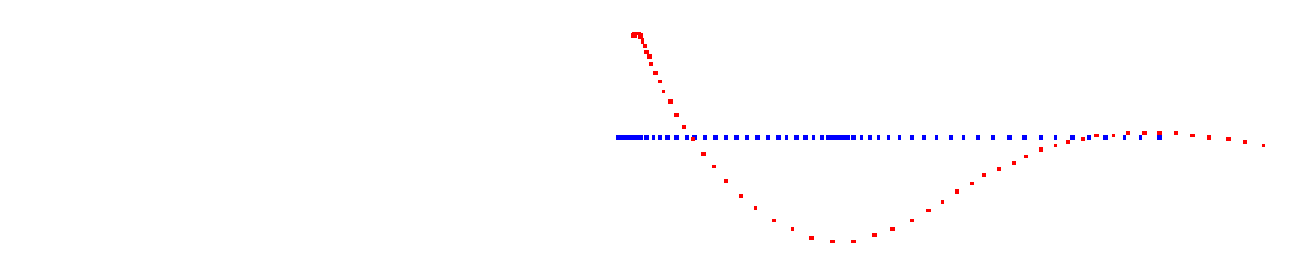
\includegraphics[width=7cm]{inestabilidadG.eps}
  \\
  \includegraphics[width=7cm]{inestabilidadC.eps}
  \caption{System dynamics with an untrained RNN controller. The first
    figure shows the pendulum trace, and the second shows the pendulum
    at $t=3.5$s.}
  \label{inestabilidad}
\end{figure}

The second experiment shows the behavior of the inverted pendulum once
the RNN controller has been evolved. Results are presented in figure
\ref{rnnSimulation}. The adaptation made by the evolutionary
algorithm, as is evident, has an important positive effect on the
controller.

\begin{figure}[t]
  \centering
  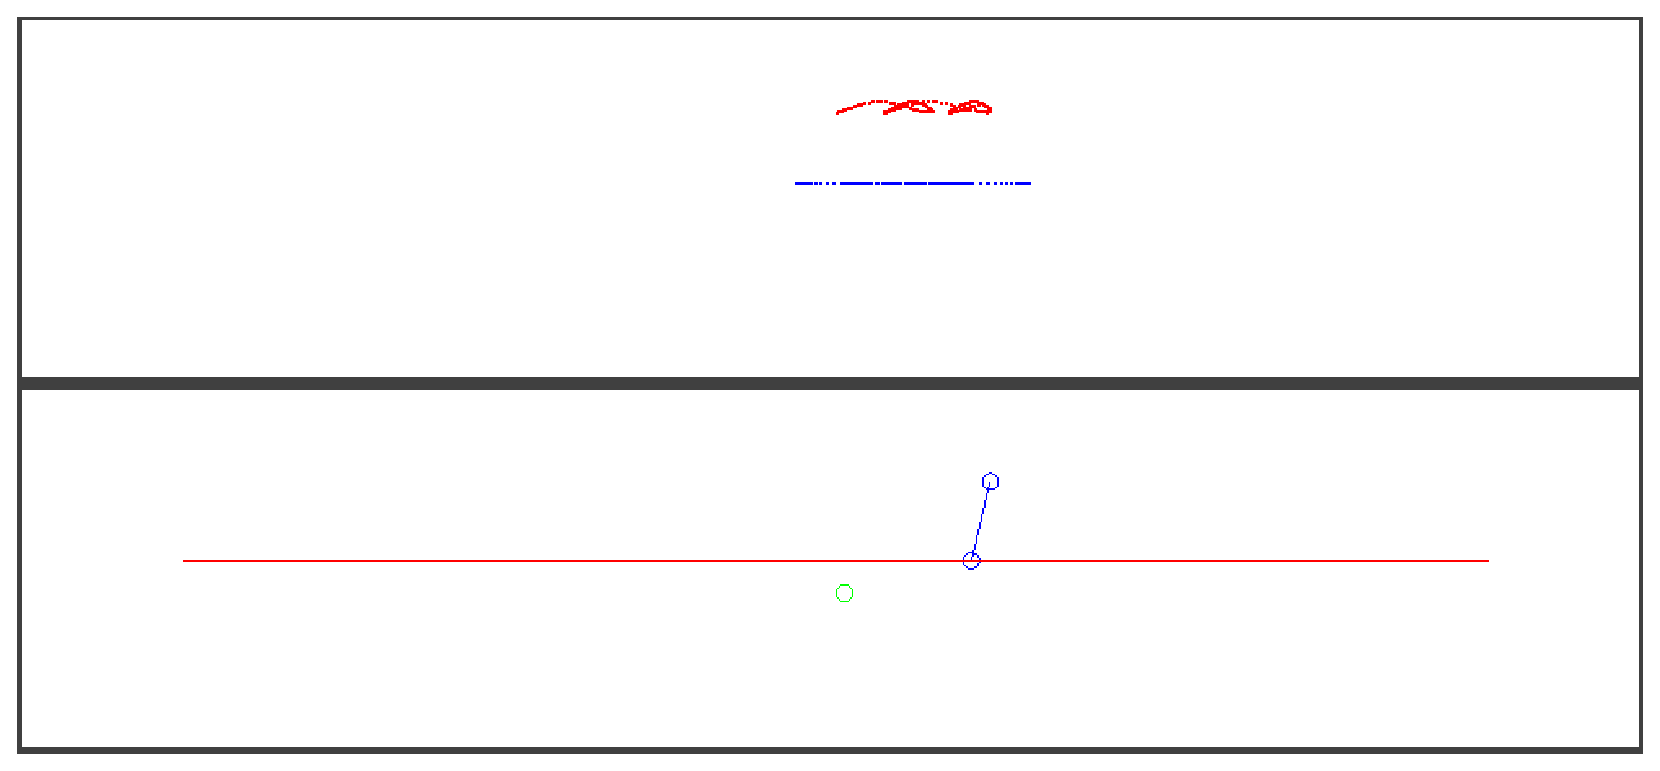
\includegraphics[width=7.5cm]{rnnSimulation.eps}
  \caption{System dynamics with a RNN controller trained. The first
    figure shows the pendulum trace and the second the pendulum at
    $t=3.5$s.}
  \label{rnnSimulation}
\end{figure}

The next three experiments were performed with: an evolved RNN
controller architecture, a (non-evolved) neural field architecture
using the processing field as output, and a (non-evolved) neural field
architecture using the input field as output (effectively omitting the
processing field in the feedback loop). Results of these three
experiments are presented comparatively in figure
\ref{fig:pendulum-plot}. In the remaining, the neural architectures
will be simply called 'input field architecture' (the architecture
omitting the processing field) and 'processing field architecture'
(the architecture using the processing field in the feedback loop).


\begin{figure}[t]
  \centering
  \includegraphics[angle=-90,width=7cm]{pendulum_thetas.eps}
  \includegraphics[angle=-90,width=7cm]{pendulum_omega.eps}
  \includegraphics[angle=-90,width=7cm]{pendulum_v.eps}
  \caption{Pendulum simulation with neural field controller between
    $t=0$s and $t=10$. Each state is coded with a position (so that
    the pendulum can be simulated as a field on its own) this way:
    $x$:0, $\theta$:1, $\dot{x}$:2, $\dot{\theta}$:3. It can be seen
    the little variation in the angular position ($\theta$). The
    discontinuity in $x$ is present because position wraps in the
    simulation so that $x=5$ is equivalent to $x=-5$.}
  \label{fig:pendulum-plot}
\end{figure}

In the upper part of figure \ref{fig:pendulum-plot}, it is shown the
behavior of the angular position state variable ($\theta$). This is
the central variable of the control task, since its minimization would
mean also a minimization of the error signal (viewed from a classical
control theory perspective). Both the recurrent neural network
architecture and the input field architecture (marked as 'input
field') show an oscillating behavior with wide movements around the
reference value ($\theta=0$). Of them, the RNN architecture has the
fastest response, but also the widest oscillations. On the contrary,
the input field architecture shows diminishing oscillations with
increasing time.

On the other hand, the processing field architecture (marked as
'processing field') presents the best performance, staying close to
the reference (with an error $|e_{\theta}|<0.5$) from $t=1.0s$
onwards.

The middle and bottom parts of figure \ref{fig:pendulum-plot} show the
state variables $\omega$ (angular velocity) and $v$ (linear
velocity). The angular velocity plot reinforces the perceptions given
by the angular position plot. It also shows that the responses of the
RNN controller and the input field architecture are softer than the
response of the processing field controller.

The linear velocity plot evidences that all controllers deviate
significantly from the initial linear position in the
experiments. This is expected, since the interest was paid only to the
balancing of the inverted pendulum, and not to its linear positioning.

While the results shown by both neural field architectures are not
ideal (none of them seems to achieve a zero error signal), their
results are certainly better than expected. This is notable,
considering that the RNN was evolved to solve the task at hand, while
the neural field architectures were manually parameterized, and there
were not applied any adaptation or evolution schemes to their
parameterization.

Processing field activations, for both neural field controllers, are
displayed in figure \ref{fig:nf-activation}. The horizontal ($x$) axis
represents the position of each element on the one-dimensional field,
and the oblique axis ($t$) represents the time elapsed. The presence
of the processing field in the feedback loop appears to act as an
integrator-like control element. On the contrary, the sole utilization
of the input field to spatially code the inputs, appears to act as a
proportional control element, causing the highly oscillating behavior
in the input field architecture. Consequently, the nonlinear coupling
between both actions, integral-like and proportional, seem to produce
the behavior presented by the processing field architecture.


\begin{figure}[t]
  \centering
  \includegraphics[angle=-90,width=7cm]{fieldPopulation_ijcnn_old.eps}
  \includegraphics[angle=-90,width=7cm]{fieldPopulation_ijcnn.eps}
  \caption{Processing fields simulation between $t=0$s and $t=10$s
    with steps $h=1/40$s and positions between $x_{min}=-10$ and
    $x_{max}=10$. In the top, the input field architecture activation
    is displayed (this activation is shown for comparing purposes but
    it is not actually used by this controller). In the bottom, the
    processing field architecture activation is displayed (actually
    used by this controller.}
  \label{fig:nf-activation}
\end{figure}

The recurrent neural network controller is expressive enough to solve
the problem at hand, but the number of parameters to configure (or in
this case to evolve) is of a quadratic order in relation to the number
of nodes (or neurons). This was not a particular problem for the
evolutionary algorithm used, but it could be a limitation if an
adaptation scheme is not applied. Furthermore, the evolutionary
parameterization applied was not able to outperform the manual
parameterization of the neural field architectures.


On the other hand, the neural field controller is a bit more complex
(in its implementation) and its simulation more costly (up to $10$
times slower than the recurrent neural network), but has some notable
advantages. The first one is its ability to self-compensate or,
equivalently, the stability of its natural dynamics, which is attained
after the setup of few parameters. The second one is its suitability
to the problem at hand, being able to solve it with a good
performance. Although there was a need for parameter configuration,
evolution was not required because the small number of parameters to
setup: basically three parameters of the kernel function and the
resting potential of the field equation - a number of parameters of
constant order in relation to the number of nodes (discrete potentials
on the neural field).


\section{Conclusions and Future Work}

In the experimentation made, the non-evolved neural field controller
was able to stabilize the inverted pendulum system, and performed
better than the evolved recurrent neural network
controller. Furthermore, the neural field has a spatial representation
which allows an interpretation of field potentials (as shown in
fig. \ref{fig:nf-activation}).

Nonetheless, in order to develop a more realistic controller of biped
walking, the mapping between the model and a biped could be detailed
\cite{Goswami08Kinematic}, or a relatively more complex model could be
used, such a 2-link model \cite{Garcia98simplest} or even of higher
order. Alternatively, a general but less detailed modelling technique
could be used, such as the Reaction Mass Pendulum
\cite{Lee07Reaction}.


More complex control problems seem to require an strategy for
parameterization of the neural field controller. This way, it is left
for future work the task of neural field evolution as it was briefly
presented in section \label{sec:properties}. Also, the capability of
neural fields to address goal-based planning problems (shown in
\cite{Bergener99Complex}), could also be used to solve higher level
control task that require, for example, multiple operation modes or
strategies.



\bibliographystyle{IEEEtran.bst}
% \bibliographystyle{natbib}
\bibliography{bibanot}

% \begin{thebibliography}{}
% \bibitem[RN] {RN} Stuart Russell and Peter Norvig (2003)
%   \textit{Artificial Intelligence: A Modern
%     Approach}. Prentice-Hall, Englewood Cliffs, NJ.
% \bibitem[Ha] {Ha} Simon Haykin (1994) \textit{Neural networks: a
%     comprehensive foundation} Macmillan.
% \bibitem[NF] {NF} Stefano Nolfi and Dario Floreano (2004)
%   \textit{Evolutionary Robotics: The Biology, Intelligence, and
%     Technology of Self-Organizing Machines} Bradford Book.
% \end{thebibliography}

\end{document}
